\boxde
\Opensolutionfile{ans}[ans/2D1-1-DEON-1]
\begin{ex}%[2D1B1-1]
    Hàm số $y=\dfrac{1}{3} x^3 - \dfrac{1}{2} x^2 +1$ đồng biến trên khoảng nào dưới đây?
    \choice
    {$(0;1) $}
    {\True $(1; +\infty) $}
    {$ (-1;1)$}
    {$(0; +\infty) $}
    \loigiai{Tập xác định $\mathscr D = \mathbb{R}$.\\
        $y'=x^2 -x $.\\
        Cho $y'=0 \Leftrightarrow \hoac{& x=0 \\&x = 1.}$\\
        Bảng biến thiên
        \begin{center}
            \begin{tikzpicture}[yscale=.8,xscale=1.5,]
                \begin{scope}[shift={(-.5,.5)}]
                    \draw[red]
                    (0,0) rectangle +(8,-5)
                    (0,-1)--+(0:8) (0,-2)--+(0:8) (1,0)--+(-90:5);
                \end{scope}
                \path
                (0,0) node{$x$} % <<< dòng 1
                ++(0:1) node{$-\infty$}
                ++(0:2) node{$0$}
                ++(0:2) node{$1$}
                ++(0:2) node{$+\infty$}
                (0,-1) node{$y'$} % <<< dòng 2
                ++(0:2) node{$+$}
                ++(0:1) node{$0$}
                ++(0:1) node{$-$}
                ++(0:1) node{$0$}
                ++(0:1) node{$+$}
                (0,-3) node{$y$} % <<< dòng 3
                ++(0:1) ++(-90:1) node (A) {$-\infty$}
                ++(0:2) ++(+90:2) node (B) {$1$}
                ++(0:2) ++(-90:2) node (C) {$\dfrac{5}{6}$}
                ++(0:2) ++(+90:2) node (D) {$+\infty$};
                \draw[-stealth,blue] (A)--(B);
                \draw[-stealth,blue] (B)--(C);
                \draw[-stealth,blue] (C)--(D);
            \end{tikzpicture}
        \end{center}
        Dựa vào bảng biến thiên ta thấy hàm số đồng biến trên khoảng $(1 ;+ \infty )$.}
\end{ex}
\begin{ex}%[2D1B1-1]
    Cho hàm số $y=-x^3 + 3x^2 -3x +1$. Mệnh đề nào dưới đây đúng?
    \choice
    {Hàm số đồng biến trên $\mathbb{R}$}
    {\True Hàm số nghịch biến trên $\mathbb{R}$}
    {Hàm số nghịch biến trên $(-\infty; 1)$ và đồng biến trên $(1; +\infty)$}
    {Hàm số đồng biến trên $(-\infty; 1)$ và nghịch biến trên $(1; +\infty)$}
    \loigiai{
        Tập xác định $\mathscr D = \mathbb{R}$.\\
        $y'= -3x^2 + 6x -3 =-3 (x-1)^2 \le 0$ với mọi $x$.\\
        Suy ra hàm số đã cho nghịch biến trên $\mathbb{R}$.}
\end{ex}
\begin{ex}%[2D1B1-1]
    Hàm số $y=2x^4 +1$ đồng biến trên khoảng nào?
    \choice
    {$\left(- \infty; - \dfrac{1}{2} \right) $}
    {\True $(0; +\infty) $}
    {$\left( - \dfrac{1}{2}; + \infty \right) $}
    {$(-\infty; 0) $}
    \loigiai{
        Ta có tập xác định $\mathscr{D} = \mathbb{R}.$\\
        $y'= 8x^3 > 0 \Leftrightarrow x>0$.\\
        Suy ra hàm số đồng biến trên $(0; + \infty)$.}
\end{ex}
\begin{ex}%[2D1B1-1]
    Khoảng đồng biến của hàm số $y=-9x^4 + \dfrac{1}{2} x^2 -\sqrt{3}$ là khoảng nào dưới đây?
    \choice
    {$(-\infty; -6) $; $(0;2)$}
    {$\left(-\dfrac{1}{6} ;0 \right) $ và $\left(0; \dfrac{1}{6} \right) $}
    {\True $\left(- \infty; -\dfrac{1}{6} \right) $ và $\left(0; \dfrac{1}{6} \right) $}
    {$ (-6;0) $ và $(6; +\infty)$}
    \loigiai{
        Tập xác định $\mathscr D = \mathbb{R}$.\\
        $y'=-36 x^3+ x$.\\
        Cho $y'=0 \Leftrightarrow \hoac{& x=0 \\&x = \pm \dfrac{1}{6} .}$\\
        Bảng biến thiên
        \begin{center}
            \begin{tikzpicture}[yscale=.75,xscale=1]
                \begin{scope}[shift={(-.5,.5)}]
                    \draw[red] (0,0) rectangle +(10,-5);
                    \draw (0,-1.2)--+(0:10) (0,-2.2)--+(0:10) (1,0)--+(-90:5);
                \end{scope}
                \path
                (-0.1,0) node{$x$} % <<< dòng 1
                ++(0:1) node{$-\infty$}
                ++(0:2) node{$- \dfrac{1}{6}$}
                ++(0:2) node{$0$}
                ++(0:2) node{$ \dfrac{1}{6}$}
                ++(0:2) node{$+\infty$}
                (0,-1.1) node{$y'$} % <<< dòng 2
                ++(0:2) node{$+$}
                ++(0:1) node{$0$}
                ++(0:1) node{$-$}
                ++(0:1) node{$0$}
                ++(0:1) node{$+$}
                ++(0:1) node{$0$}
                ++(0:1) node{$-$}
                (0,-3) node{$y$} % <<< dòng 3
                ++(0:1) ++(-90:1) node (A) {$ $}
                ++(0:2) ++(90:2) node (B) {$ $}
                ++(0:2) ++(-90:2) node (C) {$ $}
                ++(0:2) ++(+90:2) node (D) {$ $}
                ++(0:2) ++(-90:2) node (E) {$ $};
                \draw[-stealth,blue] (A)--(B);
                \draw[-stealth,blue] (B)--(C);
                \draw[-stealth,blue] (C)--(D);
                \draw[-stealth,blue] (D)--(E);
            \end{tikzpicture}
        \end{center}
        Dựa vào bảng biến thiên ta thấy hàm số đồng biến trên hai khoảng $\left(- \infty; -\dfrac{1}{6} \right) $ và $\left(0; \dfrac{1}{6} \right) $.}
\end{ex}
\begin{ex}%[2D1B1-1]
    Cho hàm số $y=f(x)$ có bảng biến thiên như sau:
    \begin{center}
        
\begin{tikzpicture}
            \tkzTabInit[nocadre,lgt=1.2,espcl=2.5,deltacl=0.6]
            {$x$/0.6,$y'$/0.6}{$-\infty$,$-2$,$0$,$+\infty$}
            \tkzTabLine{,-,0,+,0,-,}
        \end{tikzpicture}
    \end{center}
    Hàm số đồng biến trên khoảng nào dưới đây ?
    \choice
    {$(0;+\infty)$}
    {$(-\infty;-2)$}
    {$(-3;1)$}
    {\True $(-2;0)$}
    \loigiai{Trong khoảng $(-2;0)$ hàm số $y=f(x)$ có $y'=f'(x)>0$.}
\end{ex}
\begin{ex}%[2D1B1-1]
    \immini
    {
        Cho hàm số $y=f(x)$ có đồ thị như hình bên.\\
        Hàm số đã cho nghịch biến trên khoảng nào trong các khoảng dưới đây?
        \choice
        {\True $(-0,5;0,3)$}
        {$(-2;2)$}
        {$(-1,2;0,1)$}
        {$(0;2)$}
    }
    {
        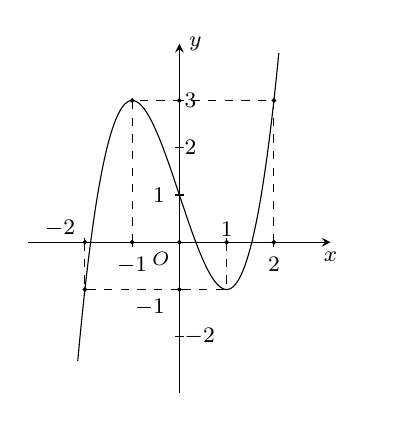
\begin{tikzpicture}[>=stealth,x=1cm,y=1cm,scale=0.6,font=\footnotesize]
            \def\a{1} % Hệ số a phải khác 0
            \def\b{0}
            \def\c{-3}
            \def\d{1}
            \def\xmin{-3}\def\xmax{3}\def\ymin{-3}\def\ymax{4}
            \draw[->] (\xmin-0.2,0)--(\xmax+0.2,0) node[below] {\footnotesize $x$};
            \draw[->] (0,\ymin-0.2)--(0,\ymax+0.2) node[right] {\footnotesize $y$};
            \foreach \x in {-1,2}\draw (\x,0.1)--(\x,-0.1) node [below] {\footnotesize $\x$};
            \foreach \x in {1}\draw (\x,0.1)--(\x,-0.1) node [above=0.1] {\footnotesize $\x$};
            \foreach \x in {-2}\draw (\x,0.1)--(\x,-0.1) node [above left] {\footnotesize $\x$};
            \foreach \y in {1}\draw (0.1,\y)--(-0.1,\y) node [left] {\footnotesize $\y$};
            \foreach \y in {2,3}\draw (0.1,\y)--(-0.1,\y) node [right=0.1] {\footnotesize $\y$};
            \foreach \y in {-2}\draw (0.1,\y)--(-0.1,\y) node [right=0.1] {\footnotesize $\y$};
            \foreach \y in {-1}\draw (0.1,\y)--(-0.1,\y) node [below left] {\footnotesize $\y$};
            \draw (0,0) node[below left]{\scriptsize $O$};
            \clip (-2.5,-2.5)rectangle(4,4);
            \draw[samples=200,smooth,domain=-2.5:2.5]plot(\x,{\a*(\x)^3+(\b)*(\x)^2+(\c)*\x+(\d)});
            \draw[dashed] (-2,0)--(-2,-1)--(0,-1);
            \draw[dashed] (-1,0)--(-1,3)--(0,3);
            \draw[dashed] (1,0)--(1,-1)--(0,-1);
            \draw[dashed] (2,0)--(2,3)--(0,3);
            \draw[fill=black] (-2,0) circle(1pt) (-2,-1) circle(1pt) (0,-1) circle(1pt) (-1,0) circle(1pt) (0,0) circle(1pt) (1,0) circle(1pt) (2,0) circle(1pt) (2,3) circle(1pt) (0,3) circle(1pt) (-1,3) circle(1pt);
        \end{tikzpicture}
    }
    \loigiai{Dựa vào đồ thị hàm số suy ra hàm số $y=f(x)$ nghịch biến trên khoảng $(-0,5;0,3)$}
\end{ex}
\begin{ex}%[2D1B1-2]
    \immini
    {
        Cho hàm số $y=f(x)$ có đồ thị như hình vẽ bên.\\
        Hàm số đã cho đồng biến trên khoảng nào dưới đây?
        \choice
        {$(0;1)$}
        {$(-\infty;1)$}
        {$(-1;1)$}
        {\True $(-1;0)$}
    }
    {
        \begin{tikzpicture}[scale=.8, font=\footnotesize, line join=round, line cap=round, >=stealth]
            \def\xmin{-2}\def\xmax{1.8}\def\ymin{-2.5}\def\ymax{0.7}
            \draw[->] (\xmin-0.2,0)--(\xmax+0.2,0) node[below] {\footnotesize $x$};
            \draw[->] (0,\ymin-0.2)--(0,\ymax+0.2) node[right] {\footnotesize $y$};
            \draw (0,0) node [below left] {\footnotesize $O$};
            \foreach \x in {,-1,1,}\draw (\x,0.1)--(\x,-0.1) node [above=0.2,scale=0.7] {\footnotesize $\x$};
            \foreach \y in {-1}\draw (0.1,\y)--(-0.1,\y) node [right=0.2,scale=0.7] {\footnotesize $\y$};
            \foreach \y in {-2}\draw (0.1,\y)--(-0.1,\y) node [below left,scale=0.7] {\footnotesize $\y$};
            \clip (-3,-3) rectangle (3,3);
            \draw[smooth,samples=200,domain=-1.64:1.64] plot (\x,{1*((\x)^4)-2*((\x)^2)-1});
            \draw[dashed] (1,0)--(1,-2)--(0,-2);
            \draw[dashed] (-1,0)--(-1,-2)--(0,-2);
            \draw[fill=white] (0,0) circle (1pt);
        \end{tikzpicture}
    }
    \loigiai{Dựa vào đồ thị hàm số suy ra hàm số $y=f(x)$ đồng biến trên các khoảng $(-1;0)$, $(1;+\infty)$.}
\end{ex}
\begin{ex}%[2D1B1-1]
    Hàm số $y=-x^{4} + 8x^{2}+6$ đồng biến trên các khoảng
    \choice
    {$(-2;0)$}
    {$(-2;2)$}
    {\True $(-\infty;-2)$}
    {$(2;+\infty)$}
    \loigiai{Tập xác định $\mathscr{D}=\mathbb{R}$.\\
        Ta có: $y'=-4x^3+16x$.\\
        Cho $y'=0 \Leftrightarrow -x^3+4x=0 \Leftrightarrow \hoac{& x=-2 \\& x= 0 \\& x=2.}$\\
        Tại $x=-2 \Rightarrow y(-2)=22$; Tại $x=0 \Rightarrow y(0)=6$; Tại $x=2 \Rightarrow y(2)=22$.\\
        Ta có bảng biến thiên
        \begin{center}
            
\begin{tikzpicture}
                \tkzTabInit[nocadre,lgt=1.2,espcl=2.5,deltacl=0.6]
                {$x$/0.6,$y'$/0.6,$y$/2}
                {$-\infty$,$-2$,$0$,$2$,$+\infty$}
                \tkzTabLine{,+,0,-,0,+,0,-,}
                \tkzTabVar{-/$-\infty$,+/$22$,-/$6$,+/$22$,-/$-\infty$}
            \end{tikzpicture}
        \end{center}
    }
\end{ex}
\begin{ex}%[2D1B1-1]
    Cho hàm số $y=\dfrac{x-2}{x+1}$ đồng biến trên khoảng
    \choice
    {$(-\infty ;+\infty)$}
    {$\mathbb{R} \backslash\{-1\}$}
    {\True $(-\infty ;-1)$}
    {$(-3 ; 3)$}
    \loigiai{Điều kiện: $ x+1 \neq 0 \Leftrightarrow x \neq -1$.\\
        Ta có: $y^{\prime}=\dfrac{3}{(x+1)^{2}} >0, \forall x \neq -1$.\\
        Bảng biến thiên
        \begin{center}
            
\begin{tikzpicture}
                \tkzTabInit[nocadre,lgt=1.2,espcl=2.5,deltacl=0.6]
                {$x$/0.6,$y'$/0.6,$y$/2}
                {$-\infty$,$-1$,$+\infty$}
                \tkzTabLine{,+,d,+,}
                \tkzTabVar{-/$1$,+D-/$+\infty$/$-\infty$,+/$1$}
            \end{tikzpicture}
    \end{center}}
\end{ex}
\begin{ex}%[2D1B1-1]
    Cho hàm số $y=\dfrac{x-1}{x+2}$. Mệnh đề nào sau đây là \textbf{đúng}?
    \choice
    {Hàm số nghịch biến trên $\mathbb{R} \backslash\{-2\}$}
    {Hàm số nghịch biến trên từng khoảng xác định của nó}
    {\True Hàm số đồng biến trên $\mathbb{R} \backslash\{-2\}$}
    {Hàm số đồng biến trên từng khoảng xác định của nó}
    \loigiai{Điều kiện: $ x+2 \neq 0 \Leftrightarrow x \neq 2$.\\
        Ta có: $y^{\prime}=\dfrac{3}{(x+2)^{2}} >0, \forall x \neq 2$.\\
        Bảng biến thiên
        \begin{center}
            
\begin{tikzpicture}
                \tkzTabInit[nocadre,lgt=1.2,espcl=2.5,deltacl=0.6]
                {$x$/0.6,$y'$/0.6,$y$/2}
                {$-\infty$,$-2$,$+\infty$}
                \tkzTabLine{,+,d,+,}
                \tkzTabVar{-/$1$,+D-/$+\infty$/$-\infty$,+/$1$}
            \end{tikzpicture}
    \end{center}}
\end{ex}
%===21
\begin{ex}%[2D1B1-1]
    Hàm số $y=2x-1+\dfrac{8}{x-1}$ đồng biến trên khoảng nào sau đây?
    \choice
    {$(-1;3)$}
    {$(-\infty;3)$}
    {\True $(-\infty;-1)$}
    {$(-1;+\infty)$}
    \loigiai{
        Tập xác định $\mathscr{D}=\mathbb{R}\setminus\{1\}$.\\
        $y'=2-\dfrac{8}{(x-1)^2}=\dfrac{2(x-1)^2-8}{(x-1)^2}$.\\
        \textbf{Cách 1:}\\
        $y'=0\Leftrightarrow (x-1)^2=4\Leftrightarrow\hoac{&x=3\\&x=-1.}$\\
        Bảng biến thiên
        \begin{center}
            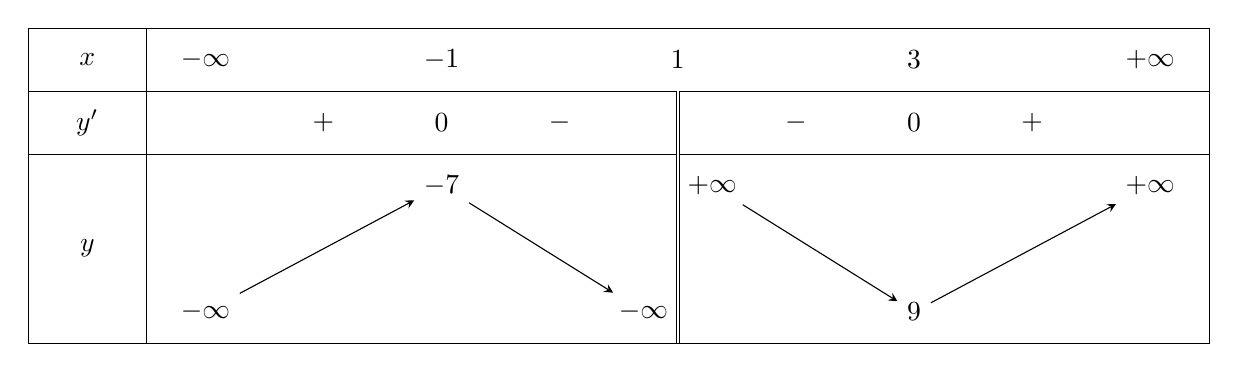
\begin{tikzpicture}[yscale=.8,xscale=1.5,]
                \begin{scope}[shift={(-.5,.5)}]
                    \draw
                    (0,0) rectangle +(10,-5)
                    (0,-1)--+(0:10) (0,-2)--+(0:10) (1,0)--+(-90:5);
                \end{scope}
                \path
                (0,0) node{$x$} % <<< dòng 1
                ++(0:1) node{$-\infty$}
                ++(0:2) node{$-1$}
                ++(0:2) node{$1$}
                ++(0:2) node{$3$}
                ++(0:2) node{$+\infty$}
                (0,-1) node{$y'$} % <<< dòng 2
                ++(0:2) node{$+$}
                ++(0:1) node{$0$}
                ++(0:1) node{$-$}
                ++(0:2) node{$-$}
                ++(0:1) node{$0$}
                ++(0:1) node{$+$}
                (0,-3) node{$y$} % <<< dòng 3
                ++(0:1) ++(-90:1) node (A) {$-\infty$}
                ++(0:2) ++(90:2) node (B) {$-7$}
                ++(0:2) ++(-90:2) node (C)[left]
                {$-\infty$}
                ++(90:2) node (D)[right]{$+\infty$}
                ++(0:2) ++(-90:2) node (E) {$9$}
                ++(0:2) ++(90:2) node (F) {$+\infty$};
                \draw[-stealth] (A)--(B);
                \draw[-stealth] (B)--(C);
                \draw[-stealth] (D)--(E);
                \draw[-stealth] (E)--(F);
                \draw[double] (5,-.5)--(5,-4.5);
            \end{tikzpicture}
        \end{center}
        \textbf{Cách 2:}\\
        $2(x-1)^2-8>0\Leftrightarrow (x-1)^2>4\Leftrightarrow \hoac{&x-1>2\\&x-1<-2} \Leftrightarrow \hoac{&x>3\\&x<-1.}$\\
        $y'>0\Leftrightarrow \hoac{&x>3\\&x<-1.}$\\
        Vậy hàm số đồng biến trên các khoảng $(-\infty; -1)$ và $(3;+\infty)$.
    }
\end{ex}
%===22
\begin{ex}%[2D1B1-1]
    Hàm số $y=\dfrac{x^2-3x}{x+1}$ nghịch biến trên khoảng nào sau đây?
    \choice
    {$(-3;1)$}
    {\True $(-3;-1)$}
    {$(-\infty;-3)$}
    {$(1;+\infty)$}
    \loigiai{
        Tập xác định $\mathscr{D}=\mathbb{R}\setminus\{-1\}$.\\
        $y'=\dfrac{x^2+2x-3}{(x+1)^2}$.\\
        \textbf{Cách 1:}\\
        $y'=0\Leftrightarrow \hoac{&x=1\\&x=-3.}$\\
        Bảng biến thiên
        \begin{center}
            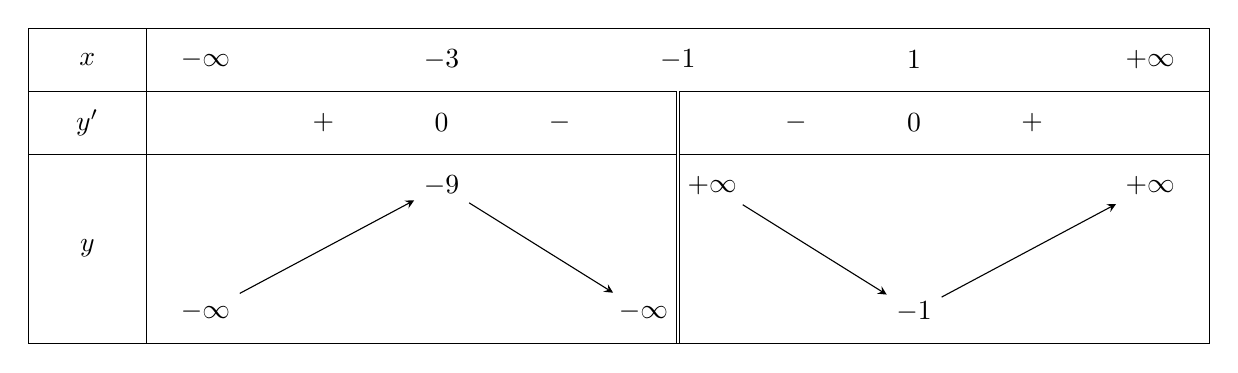
\begin{tikzpicture}[yscale=.8,xscale=1.5,]
                \begin{scope}[shift={(-.5,.5)}]
                    \draw
                    (0,0) rectangle +(10,-5)
                    (0,-1)--+(0:10) (0,-2)--+(0:10) (1,0)--+(-90:5);
                \end{scope}
                \path
                (0,0) node{$x$} % <<< dòng 1
                ++(0:1) node{$-\infty$}
                ++(0:2) node{$-3$}
                ++(0:2) node{$-1$}
                ++(0:2) node{$1$}
                ++(0:2) node{$+\infty$}
                (0,-1) node{$y'$} % <<< dòng 2
                ++(0:2) node{$+$}
                ++(0:1) node{$0$}
                ++(0:1) node{$-$}
                ++(0:2) node{$-$}
                ++(0:1) node{$0$}
                ++(0:1) node{$+$}
                (0,-3) node{$y$} % <<< dòng 3
                ++(0:1) ++(-90:1) node (A) {$-\infty$}
                ++(0:2) ++(90:2) node (B) {$-9$}
                ++(0:2) ++(-90:2) node (C)[left]
                {$-\infty$}
                ++(90:2) node (D)[right]{$+\infty$}
                ++(0:2) ++(-90:2) node (E) {$-1$}
                ++(0:2) ++(90:2) node (F) {$+\infty$};
                \draw[-stealth] (A)--(B);
                \draw[-stealth] (B)--(C);
                \draw[-stealth] (D)--(E);
                \draw[-stealth] (E)--(F);
                \draw[double] (5,-.5)--(5,-4.5);
            \end{tikzpicture}
        \end{center}
        \textbf{Cách 2:}\\
        $x^2+2x-3<0\Leftrightarrow -3<x<1$.\\
        $y'<0\Leftrightarrow \hoac{&-3<x<-1\\&-1<x<1.}$\\
        Vậy hàm số nghịch biến trên các khoảng $(-3; -1)$ và $(-1;1)$.
    }
\end{ex}
%===30
\begin{ex}%[2D1B1-1]
    Hàm số $y=\sqrt{x^2-4x+3}$ nghịch biến trên khoảng nào sau đây?
    \choice
    {$(3;+\infty)$}
    {$(1;3)$}
    {\True $(-\infty;1)$}
    {$(-\infty;3)$}
    \loigiai{
        Tập xác định $\mathscr{D}=(-\infty;1]\cup [3;+\infty)$.\\
        $y'=\dfrac{2x-4}{2\sqrt{x^2-4x+3}}$.\\
        \textbf{Cách 1:}\\
        $2x-4=0\Leftrightarrow x=2$.\\
        Bảng biến thiên
        \begin{center}
            \begin{tikzpicture}[yscale=.8,xscale=1.5,]
                \begin{scope}[shift={(-.5,.5)}]
                    \fill[pattern=north east lines,pattern color=violet](3.5,-1) rectangle +(2,-4);
                    \draw
                    (0,0) rectangle +(8,-5)
                    (0,-1)--+(0:8) (0,-2)--+(0:8) (1,0)--+(-90:5);
                \end{scope}
                \path
                (0,0) node{$x$} % <<< dòng 1
                ++(0:1) node{$-\infty$}
                ++(0:2) node{$1$}
                ++(0:1) node{$2$}
                ++(0:1) node{$3$}
                ++(0:2) node{$+\infty$}
                (0,-1) node{$y'$} % <<< dòng 2
                ++(0:2) node{$-$}
                ++(0:2)
                ++(0:2) node{$+$}
                (0,-3) node{$y$} % <<< dòng 3
                ++(0:1) ++(+90:1) node (A) {$+\infty$}
                ++(0:2) ++(-90:2) node (B) {$0$}
                ++(0:2) node (C) {$0$}
                ++(0:2) ++(+90:2) node (D) {$+\infty$};
                \draw[-stealth] (A)--(B);
                \draw[-stealth] (C)--(D);
                \draw[double] (3,-.5)--(3,-1.5) (5,-.5)--(5,-1.5);
            \end{tikzpicture}
        \end{center}
        \textbf{Cách 2:}\\
        $2x-4<0 \Leftrightarrow x<2$.\\
        $y'<0 \Leftrightarrow x<1$.\\
        Vậy hàm số nghịch biến trên khoảng $(-\infty;1)$.
    }
\end{ex}
\begin{ex}%[2D1B1-1]
    Tìm khoảng đồng biến của hàm số $ f(x)$, biết $f'(x)=(x-1)\left(x^2-5x+4\right),\forall x\in\mathbb{R}$.
    \choice
    {$(1 ; 4)$ }
    { \True $(4 ;+\infty)$}
    { $(1 ;+\infty)$ }
    { $(-\infty ; 4)$}
    \loigiai
    {
        Cho $f'(x)=0 \Rightarrow (x-1)\left(x^2-5x+4\right)=0 \Leftrightarrow \hoac{&x=1\\ &x=4.}$\\
        Bảng xét dấu $f'(x)$
        \begin{center}
            \begin{tikzpicture}
                \tkzTabInit[nocadre=false,lgt=2,espcl=2,deltacl=0.5]{$x$/1 ,$f'(x)$/1 }
                {$-\infty$ , $1$ , $4$ , $+\infty$}
                \tkzTabLine{ , - , z , - , z , + }
            \end{tikzpicture}
        \end{center}
        Vậy hàm số đồng biến trên $(4;+\infty)$.
    }
\end{ex}
\begin{ex}%[2D1B1-1]
    Tìm khoảng nghịch biến của hàm số $f(x)$,
    biết $f'(x)=(x-3)^2\left(x^8-8\right),\forall x\in\mathbb{R}$.
    \choice
    { $(-\infty ; 3)$}
    {$(3 ;+\infty)$ }
    { $(2 ; 3)$ }
    {\True $(-\infty ; 2)$}
    \loigiai
    {
        Cho $f'(x)=0 \Rightarrow (x-3)^2\left(x^3-8\right)=0 \Leftrightarrow \hoac{&x=3\\ &x=2.}$\\
        Bảng xét dấu $f'(x)$
        \begin{center}
            \begin{tikzpicture}
                \tkzTabInit[nocadre=false,lgt=2,espcl=2,deltacl=0.5]{$x$/1 ,$f'(x)$/1 }
                {$-\infty$ , $2$ , $3$ , $+\infty$}
                \tkzTabLine{ , - , z , + , z , + }
            \end{tikzpicture}
        \end{center}
        Vậy hàm số nghịch biến trên $(-\infty; 2)$.
    }
\end{ex}
\begin{ex}%[2D1B1-1]
    \immini{Cho hàm số đa thức $ f(x)$ có đồ thị $y=f'(x)$ như hình vẽ bên dưới. Tìm khẳng định đúng.
        \choice
        { Hàm số $f(x)$ nghịch biến trên $(-\infty ; 0)$}
        {Hàm số $f(x)$ đồng biến trên $(0 ;+\infty)$ }
        {\True Hàm số $f(x)$ đồng biến trên $(1 ;+\infty)$}
        {Hàm số $f(x)$ nghịch biến trên $(-\infty ;-1)$}}{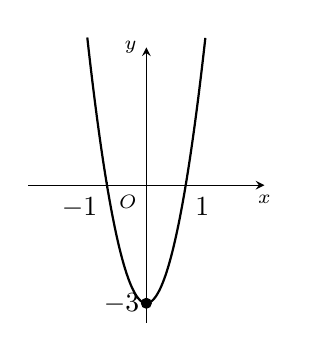
\begin{tikzpicture}[>=stealth,x=.5cm,y=.5cm]
            \def\a{3} % Hệ số a phải khác 0
            \def\b{0}
            \def\c{-3}
            \draw[->] (-3,0) -- (3,0) node[below] {\scriptsize $x$};
            \draw[->] (0,-3.5) -- (0,3.5) node[left] {\scriptsize $y$};
            \draw[thin] (-1,1pt)--(-1,-1pt) node [below left] {$-1$} (1,1pt)--(1,-1pt) node [below right] {$1$} (-1pt,-3 )--(1pt,-3) node [left] {$-3$} ;
            \draw (0,0)node[below left]{\scriptsize $O$};
            \pgfmathsetmacro\xdinh{-(\b)/2*(\a)}
            \pgfmathsetmacro\ydinh{(4*(\a)*(\c)-(\b)^2)/(4*(\a))}
            \fill[dashed] (\xdinh,\ydinh)circle(2pt) edge (\xdinh,0) edge (0,\ydinh);
            \clip (-3,-3.5)rectangle(3.6,4);
            \draw[thick,samples=150,smooth,domain=-1.5:1.5] plot(\x,{\a*(\x)^2+(\b)*\x+(\c)});
    \end{tikzpicture}}
    \loigiai
    {
        Dựa vào đồ thị ta thấy $f'(x)> 0 $ trên các khoảng $(-\infty; -1), (1;+\infty)$ nên đồng biến trên các khoảng đó, $f'(x)<0$ trên $(-1;1)$ nên nghịch biến trên đó.
    }
\end{ex}
\begin{ex}%[2D1B1-1]
    Cho hàm số $ y = f(x)$ có $f'(x)=\left(x^2-1\right)(x+1)(5-x), \forall x\in\mathbb{R}$. Mệnh đề nào sau đây đúng ?
    \choice
    {$f(1)<f(4)<f(2)$}
    {\True $f(1)<f(2)<f(4)$}
    {$f(2)<f(1)<f(4)$}
    {$f(4)<f(2)<f(1)$}
    \loigiai
    {
        Cho $f'(x)=0 \Rightarrow \left(x^2-1\right)(x+1)(5-x)=0 \Leftrightarrow \hoac{&x=-1\\ &x=1\\ &x=5.} $\\
        Bảng xét dấu $f'(x)$
        \begin{center}
            \begin{tikzpicture}
                \tkzTabInit[nocadre=false,lgt=2,espcl=2,deltacl=0.5]{$x$/1 ,$f'(x)$/1 }
                {$-\infty$ , $-1$ , $1$ , $5$ , $+\infty$}
                \tkzTabLine{ , - , z , - , z , + , z , - }
            \end{tikzpicture}
        \end{center}
        Do đó hàm số đồng biến trên khoảng $(1 ; 5)$.\\
        Vậy $f(1)<f(2)<f(4)$.
    }
\end{ex}
\begin{ex}%[2D1Y1-2]
    Cho hàm số $y=f(x)$ có bảng biến thiên như hình bên dưới. Mệnh đề nào sau đây \textbf{sai}?
    \begin{center}
        
\begin{tikzpicture}
            \tkzTabInit[lgt=1,espcl=2.5,deltacl=0.6]
            {$x$ /0.6,$y'$ /0.6,$y$ /1.5}
            {$-\infty$,$1$,$5$,$+\infty$}
            \tkzTabLine{,+,$0$,-,d,-,}
            \tkzTabVar{-/$-\infty$,+/$3$,-D+/$-\infty$/$+\infty$,-/$4$}
        \end{tikzpicture}
    \end{center}
    \choice
    {Hàm số $y=f(x)$ đồng biến trên khoảng $(-\infty;1)$}
    {Hàm số $y=f(x)$ nghịch biến trên khoảng $(1;2)$}
    {Hàm số $y=f(x)$ đồng biến trên khoảng $(-2;0)$}
    {\True Hàm số $y=f(x)$ nghịch biến trên khoảng $(4;6)$}
    \loigiai{
        Từ bảng biến thiên ta có
        \begin{itemize}
            \item Hàm số đồng biến trên khoảng $(-\infty;1)$.
            \item Hàm số nghịch biến trên khoảng $(1;5)$ và $(5;+\infty)$.
        \end{itemize}
    }
\end{ex}
\begin{ex}%[2D1Y1-2]
    Cho hàm số $y=f(x)$ có bảng biến thiên như hình bên dưới. Mệnh đề nào sau đây \textbf{đúng}?
    \begin{center}
        \begin{tikzpicture}
            \tkzTabInit[lgt=1,espcl=2.5,deltacl=0.6]
            {$x$ /0.6,$y'$ /0.6,$y$ /1.5}
            {$-\infty$,$-1$,$2$,$5$,$+\infty$}
            \tkzTabLine{,+,$0$,+,d,+,$0$,-,}
            \draw (N13)node[above](A){$-2$} ($(N13)!0.5!(N32) +(0,0.1)$) node(B){$1$} (N32)[below left]node(C){$+\infty$};
            \foreach \x/\y in {A/B,B/C}
            {\draw[-stealth] (\x)--(\y);}
            \draw[double] ([yshift=-0.5mm]N32)--(N33);
            \draw (N33)node[above right](D){$-\infty$} (N42)[below]node(E){$3$} (N53)[above]node(F){$-\infty$};
            \foreach \m/\n in {D/E,E/F}
            {\draw[-stealth] (\m)--(\n);}
        \end{tikzpicture}
    \end{center}
    \choice
    {Hàm số đã cho không đồng biến trên khoảng $(-\infty;2)$}
    {Hàm số đã cho không nghịch biến trên khoảng $(5;6)$}
    {\True Hàm số đã cho không đồng biến trên khoảng $(-1;5)$}
    {Hàm số đã cho không nghịch biến trên khoảng $(5;+\infty)$}
    \loigiai{
        Từ bảng biến thiên ta có
        \begin{itemize}
            \item Hàm số đồng biến trên khoảng $(-\infty;2)$ và $(2;5)$.
            \item Hàm số nghịch biến trên khoảng $(5;+\infty)$.
        \end{itemize}
    }
\end{ex}
\begin{ex}%[2D1B1-1]
    Cho hàm số $y=a x^{4}+b x^{2}+c,$ $(a \neq 0)$ có bảng biến thiên bên dưới. Hỏi đó là hàm số nào?
    \begin{center}
        
\begin{tikzpicture}
            \tkzTabInit[nocadre,lgt=1.2,espcl=2.5,deltacl=0.6]
            {$x$/0.6,$y'$/0.6,$y$/1.5}
            {$-\infty$,$-1$,$0$,$1$,$+\infty$}
            \tkzTabLine{,-,0,+,0,-,0,+,}
            \tkzTabVar{+/$+\infty$,-/$1$,+/$2$,-/$1$,+/$+\infty$}
        \end{tikzpicture}
    \end{center}
    \choice
    {$y=-x^{4}+2 x^{2}+2$}
    {\True $y=x^{4}-2 x^{2}+2$}
    {$y=x^{4}-2 x-2$}
    {$y=-x^{4}+2 x-2$}
    \loigiai{Ta có: $y'=4ax^3+2bx$.\\
        Dựa vào bảng biến thiên, ta thấy đồ thị đi qua các điểm $(-1;1)$, $(0;2)$, $(1;0)$, các điểm này là các điểm cực trị của hàm số.\\
        $\Rightarrow \heva{& y(0)=2\\& y(\pm 1)=1 \\& y'(\pm 1)=0} \Leftrightarrow \heva{ & c= 2 \\& a+b+c=1\\&2a+b=0} \Leftrightarrow \heva{& c=2 \\& b=-2\\& a=1.}$}
\end{ex}
\begin{ex}%Câu 99
    Cho hàm số $y = -x^3-mx^2 +(4m+9)x+5$ với $m$ là tham số. Có bao nhiêu giá trị nguyên của $m$ để hàm số đã cho nghịch biến trên khoảng $(-\infty;+\infty)$?
    \choice
    {\True $7$}
    {$4$}
    {$6$}
    {$5$}
    \loigiai{Ta có $ y'=-3x^2-2mx+4m+9.$\\
        Hàm số nghịch biến trên khoảng $(-\infty;+\infty) \Leftrightarrow \Delta ' \le 0 \Leftrightarrow m^2+12m+27 \le 0 \Leftrightarrow -9\le m \le -3.$\\
        Vậy có 7 giá trị nguyên của $m$.}
\end{ex}
\begin{ex}%Câu 100
    Có bao nhiêu giá trị nguyên của tham số $m$ để hàm số $y=x^3 -mx^2 + 3x-1$ đồng biến trên khoảng $(-\infty;+\infty)$?
    \choice
    {$8$}
    {$4$}
    {\True $7$}
    {Vô số}
    \loigiai{
        Ta có $ y'=3x^2-2mx+3.$\\
        Hàm số đồng biến trên khoảng $(-\infty;+\infty) \Leftrightarrow \Delta ' \le 0 \Leftrightarrow m^2-9 \le 0 \Leftrightarrow -3\le m\le 3.$\\
        Vậy có 7 giá trị nguyên của $m$.}
\end{ex}
\begin{ex}%Câu 86
    Cho hàm số $y=\dfrac{x+m}{x-1}$. Có bao nhiêu giá trị nguyên của tham số $m$ thuộc khoảng $(-10;10)$ để hàm số đã cho đồng biến trên từng khoảng xác định của nó?
    \choice
    {\True 8}
    {9}
    {10}
    {11}
    \loigiai{
        Tập xác định $\mathit{D}=\mathbb{R} \backslash \{1\}.$\\
        Ta có $y'=\dfrac{-1-m}{(x-1)^2}.$\\
        Ta cần $y'>0, \forall x \in \mathit{D} \Leftrightarrow -1-m >0\Leftrightarrow m <-1.$\\
        mà $m \in (-10;10) \Rightarrow$ do đó $m$ có 8 giá trị nguyên.
    }
\end{ex}
\begin{ex}%Câu 87
    Cho hàm số $y=\dfrac{mx+4m}{x+m}$ với $m$ là tham số. Gọi $S$ là tập hợp tất cả các giá trị nguyên của $m$ để hàm số đã cho nghịch biến trên các khoảng xác định. Số phần tử của $S$ là
    \choice
    {5}
    { Vô số}
    {4}
    {\True 3}
    \loigiai{
        Tập xác định $\mathit{D}=\mathbb{R} \backslash \{-m\}.$\\
        Ta có $y'=\dfrac{m^2-4m}{(x+m)^2}.$\\
        Ta cần $y'<0, \forall x \in \mathit{D} \Leftrightarrow m^2-4m <0\Leftrightarrow 0<m<4.$\\
        Vậy có 3 giá trị $m$.}
\end{ex}
\begin{ex}%Cậu 90
    Có bao nhiêu giá trị nguyên của tham số $m$ để hàm số $y=\dfrac{x+2}{x+5m}$ đồng biến trên khoảng $(-\infty;-10)$?
    \choice
    {\True $2$}
    { Vô số}
    {$1$}
    {$3$}
    \loigiai{
        Tập xác định $\mathit{D}=\mathbb{R} \backslash \{-5m\}.$\\
        Ta có $y'=\dfrac{5m-2}{(x+5m)^2}.$\\
        Ta cần $y'>0, \forall x \in (-\infty;-10) \Leftrightarrow \heva{&5m-2>0\\ &x<-10} \Leftrightarrow \heva{&m>\dfrac{2}{5}\\ &-5m\ge -10} \Leftrightarrow \heva{&m>\dfrac{2}{5}\\ &m\le 2.}\Leftrightarrow \dfrac{2}{5}<m\le 2.$\\
        Vậy có 2 giá trị $m$ thỏa đề bài.}
\end{ex}
\begin{ex}%Câu 91
    Có bao nhiêu giá trị nguyên của tham số $m$ để hàm số $y=\dfrac{x+6}{x+5m}$ nghịch biến trên khoảng $(10;+\infty)$?
    \choice
    {$3$}
    {Vô số}
    {\True $4$}
    {$5$}
    \loigiai{
        Tập xác định $\mathit{D}=\mathbb{R} \backslash \{-5m\}.$\\
        Ta có $y'=\dfrac{5m-6}{(x+5m)^2}.$\\
        Ta cần $y'<0, \forall x \in (10;+\infty) \Leftrightarrow \heva{&5m-6<0\\ &x>10} \Leftrightarrow \heva{&m<\dfrac{6}{5}\\ &-5m\le 10} \Leftrightarrow \heva{&m<\dfrac{6}{5}\\ &m\ge -2.}$\\
        Vậy có 4 giá trị $m$.}
\end{ex}
\begin{ex}%Câu 95
    Tập hợp tất cả các giá trị của tham số $m$ sao cho hàm số $y =\dfrac{\tan x-2}{\tan x-m}$ đồng biến trên khoảng $\left(0;\dfrac{\pi}{4}\right)$.
    \choice
    {$(2;+\infty)$}
    {$(-\infty;0]$}
    {$[1;2)$}
    {\True $(-\infty;0] \cup [1;2)$}
    \loigiai{
        Ta có $y'=\dfrac{-m+2}{(\tan x-m)^2} \cdot \dfrac{1}{\cos^2x}.$\\
        Hàm số đồng biến trên khoảng $\left(0;\dfrac{\pi}{4}\right) \Leftrightarrow \heva{&-m+2>0\\&\tan x \ne m, \forall x \in \left(0;\dfrac{\pi}{4}\right)}\Leftrightarrow \heva{&m<2\\&m \notin \left(\tan 0;\tan \dfrac{\pi}{4}\right)=(0;1)} \\
        \Leftrightarrow \heva{&m<2\\& \hoac{&m \ge 1\\ & m \le 0.}}$}
\end{ex}
\begin{ex}%[2D1G1-3]
    \immini{Cho hàm số bậc bốn $y=f(x)$ có $f\left(-\dfrac{3}{2}\right)<2$ và $f(1)=0$. Biết hàm số $y=f'(x)$ có đồ thị như hình vẽ. Hàm số $g(x)=\left| f\left(1-\dfrac{x}{2}\right)-\dfrac{x^2}{8}\right|$ đồng biến trên khoảng nào dưới đây?
            \choice
        {$(-\infty;-4)$}
        {$(5;+\infty)$}
        {$(2;4)$}
        {$(2;4)$}
    }{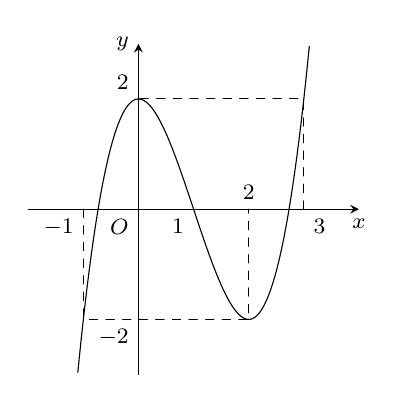
\begin{tikzpicture}[>=stealth, line join=round, line cap=round, font=\footnotesize, scale=.7]
            \def\a{1} % Hệ số a phải khác 0
            \def\b{-3}
            \def\c{0}
            \def\d{2}
            \draw[->] (-2,0) -- (4,0)node[below]{$x$};
            \draw[->] (0,-3) -- (0,3) node[left] {$y$};
            \draw (0,0)node[below left]{$O$} (1,0)node[below left]{$1$};
            \draw[dashed] (-1,0)node[below left]{$-1$}|-(0,-2)node[below left]{$-2$}-|(2,0)node[above]{$2$}
            (0,2)node[above left]{$2$} (3,0)node[below right]{3}|-(0,2);
            \draw[samples=150,smooth,domain=-1.1:3.1] plot(\x,{\a*(\x)^3+(\b)*(\x)^2+(\c)*\x+(\d)});
    \end{tikzpicture}}
\end{ex}
\begin{ex}%[2D1G1-3]
    Cho hàm số $y=f(x)$ có bảng biến thiên như hình vẽ bên dưới. Có bao nhiêu giá trị nguyên của tham số $m\in \left[-20;20\right]$ để hàm số $y=f(2\tan x+m)$ đồng biến trên khoảng $\left(0;\dfrac{\pi}{4}\right)$?
    \begin{center}
        
\begin{tikzpicture}
            \tkzTabInit[lgt=1.5,espcl=2,deltacl=.5]
            {$x$ /.7, $y'$ /.7,$y$ /2}
            {$-\infty$,$-3$,$0$,$+\infty$}
            \tkzTabLine{,-,$0$,+,$0$,-,}
            \tkzTabVar{-/$-\infty$,+/,-/,+/$+\infty$}
        \end{tikzpicture}
    \end{center}
    \choice
    {$36$}
    {$35$}
    {\True $37$}
    {$38$}
    \loigiai{
        Đặt $t=2\tan x +m, x\in \left(0;\dfrac{\pi}{4}\right)\Rightarrow t\in (m;m+2)$ và $ t'=\dfrac{2}{\cos ^2x}>0, \forall x\in \left(0;\dfrac{\pi}{4}\right)$.
        \\
        $f(2\tan x +m)$ đồng biến trên khoảng $\left(0;\dfrac{\pi}{4}\right)$
        \\
        $\Leftrightarrow f(t)$ đồng biến trên khoảng $(m;m+2)$
        \\
        $\Leftrightarrow f'(t)\geq , \forall x\in (m;m+2)$
        \\
        $\Leftrightarrow \hoac{&m+2\leq -3\\&m\geq 0}\Leftrightarrow \hoac{&m\leq 5\\&m\geq 0.}$
        \\
        Mặt khác $m\in [-20;20]$ nên có $37$ giá trị của $m$ thỏa yêu cầu đề bài.
    }
\end{ex}
\begin{ex}%[2D1G1-3]
    Cho hàm số $f(x)=|x^3-(2m-5)x+2018|$. Có bao nhiêu giá trị nguyên của tham số $m$ thuộc $[-2024;2024]$ để hàm số đồng biến trên $(1;3)$?
    \choice
    {\True $3042$}
    {$4039$}
    {$0$}
    {$2023$}
    \loigiai{
        $y=|x^3-(2m-5)x+2018| \Rightarrow y'=\dfrac{(3x^2-2m+5)[x^3-(2m-5)x+2018]}{|x^3-(2m-5)x+2018|}$.
        \\
        Hàm số đồng biến trên $(1;3)$ khi $y'\geq 0, \forall x\in (1;3)$.
        \\
        $\Leftrightarrow (3x^2-2m+5)[x^3-(2m-5)x+2018] \geq 0, \forall x\in (1;3)$
        \\
        $\Leftrightarrow \hoac{&\heva{&3x^2-2m+5\geq 0\\&x^3-(2m-5)x+2018\geq 0}\\&\heva{&3x^2-2m+5\leq 0\\&x^3-(2m-5)x+2018\leq 0}}, \forall x\in (1;3)
        \Leftrightarrow \hoac{&\heva{&3x^2-2m+5\geq 0\\&x^3-(2m-5)x+2018\geq 0}\\&\heva{&3x^2-2m+5\leq 0\\&x^3-(2m-5)x+2018\leq 0}}, \forall x\in (1;3).
        $
        \\
        $\Leftrightarrow \hoac{&\heva{&2m\leq 3x^2+5\\&2m\leq \dfrac{x^3+2018}{x}+5}
            \\&\heva{&2m\geq 3x^2+5\\&2m\geq \dfrac{x^3+2018}{x}+5}}, \forall x\in (1;3) \Leftrightarrow \hoac{&m \leq 4\\&m\geq 1012.}$
        \\
        Vậy có $3042$ giá trị của $m$ thỏa mãn yêu cầu đề bài.
    }
\end{ex}
\Closesolutionfile{ans}
%\indapan{10}{ans/2D1-1-DEON-1}
